\begin{frame}{Last lecture: a small MLP for computer vision}

  \begin{columns}
    \begin{column}{0.48\textwidth}
      \begin{figure}
        \includegraphics[width=0.9\textwidth]{neuron_01}
      \end{figure}
    \end{column}
    \begin{column}{0.48\textwidth}
      \begin{align*}
        128 \times 128 \times 3 & = 49152 \\
        16 \times 16 \times 36 & = 9216 \\
        \rightarrow 49152 \cdot 9216 + 9216 \cdot 10 & = 453076992 \approx 450 \cdot 10^{6}
      \end{align*}
    \end{column}
  \end{columns}

  \note{
    \begin{itemize}
      \item A small MLP with feature vector comparable to HOG.
      \item Input: an rgb image relatively low resolution\\
            $\rightarrow 128\times128\times3 = 49152 $
      \item Hidden layer: comparable to HOG with 36 dim feature vector computed from $8\times 8$ patches \\
            $\rightarrow$ $16\times16\times36 = 9216$
      \item Output neurons for e.g. 10 object classes \\
            $\rightarrow 49152 \cdot 9216 + 9216 \cdot 10 = 453076992 \approx 450 million$ parameters\\
    \end{itemize}

  }
\end{frame}


\begin{frame}

  \begin{columns}
    \begin{column}{0.48\textwidth}
      \begin{figure}
        \includegraphics[width=0.9\textwidth, angle=-90]{cow_00}
      \end{figure}
    \end{column}
    \begin{column}{0.48\textwidth}
      Do we need to connect all the pixels?
      \begin{figure}
        \includegraphics[width=0.85\textwidth]{convnet_00}
      \end{figure}

    \end{column}
  \end{columns}

  \note{
    \begin{itemize}
      \item Can we use knowledge about image statistics to reduce the number of connections?
    \end{itemize}
  }
\end{frame}


\begin{frame}{Convolutional Layers: locality}
  \begin{figure}
    \includegraphics[width=0.45\textwidth]{convnet_00}
    \includegraphics[width=0.45\textwidth]{convnet_01}
  \end{figure}

  \note{
    \begin{itemize}
      \item Assumption: local regions to be processed together, regions far apart not related
    \end{itemize}
  }
\end{frame}


\begin{frame}{Convolutional Layers: weight sharing}
  \begin{figure}
    \includegraphics[width=0.45\textwidth]{convnet_00}
    \includegraphics[width=0.45\textwidth]{convnet_02}
  \end{figure}
  \note{
    \begin{itemize}
      \item Assumption: image processing should not vary with image region.
    \end{itemize}
  }
\end{frame}


\begin{frame}{Convolutional Layers: feature maps}
  \begin{figure}
    \includegraphics[width=0.55\textwidth]{convnet_03}
  \end{figure}
  \note{
    \begin{itemize}
      \item Instead we can connect multiple neurons to every dimension of the input.
    \end{itemize}
  }
\end{frame}


\begin{frame}{Convolutional Layers: kernel in 2d}
  \begin{figure}
    \includegraphics[width=0.55\textwidth]{convnet_2d_00}
  \end{figure}
  \note{
    \begin{itemize}
      \item A convolutional layer corresponds to a convolution with a filter kernel plus non linearity.
    \end{itemize}
  }
\end{frame}


\begin{frame}{Convolutional Layers: padding}
  \begin{figure}
    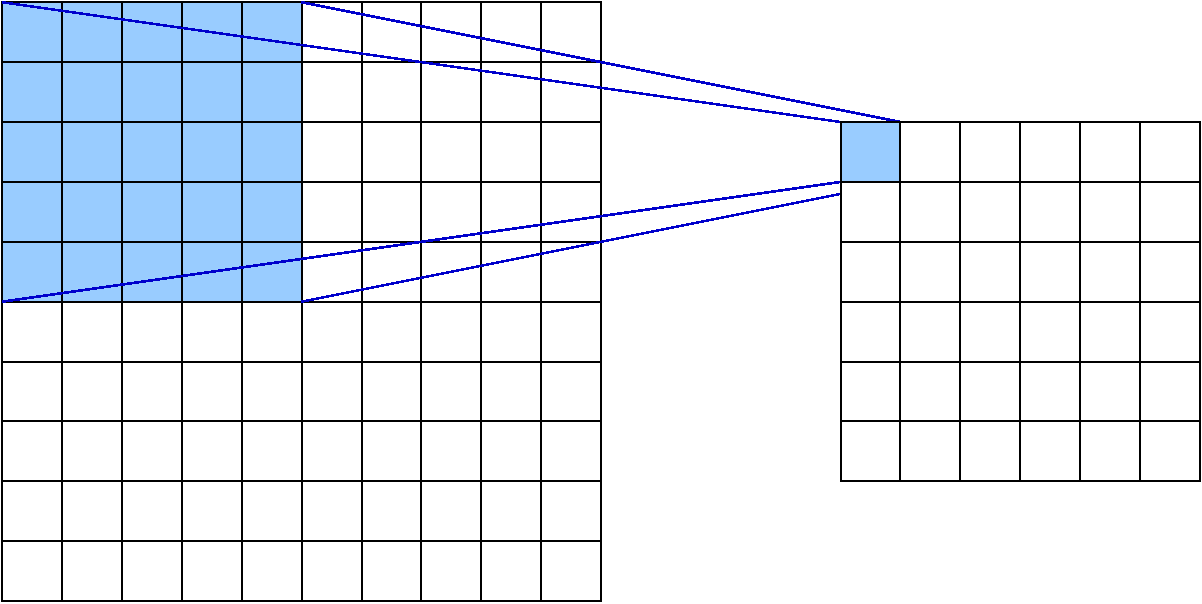
\includegraphics[width=0.55\textwidth]{convnet_2d_01}
  \end{figure}
  \note{
    \begin{itemize}
      \item We loose $\frac{1}{2}$ kernel size pixels at the image boarder.
    \end{itemize}
  }
\end{frame}


\begin{frame}{Convolutional Layers: padding}
  \begin{figure}
    \includegraphics[width=0.55\textwidth]{convnet_2d_padding}
  \end{figure}
  \note{
    \begin{itemize}
      \item Usually we pad image boarder to keep image size.
    \end{itemize}
  }
\end{frame}


\begin{frame}{Convolutional Layers: strides}
  \begin{figure}
    \includegraphics[width=0.55\textwidth]{convnet_2d_strides_00}
  \end{figure}
  \note{
    \begin{itemize}
      \item The number of pixels in between neurons is called stride.
    \end{itemize}
  }
\end{frame}


\begin{frame}{Convolutional Layers: strides}
  \begin{figure}
    \includegraphics[width=0.55\textwidth]{convnet_2d_strides_01}
  \end{figure}

  \note{
    \begin{itemize}
      \item With strides $>1$ we can downsample the image to lower resolution.
    \end{itemize}
  }
\end{frame}


\begin{frame}{Im2Col}
  \begin{figure}
    \includegraphics[width=0.55\textwidth]{convnet_im2col_00}
  \end{figure}

  \note{
    \begin{itemize}
      \item To formulate the convolutions as matrix operations, the image pixels are duplicated and rearranged.
    \end{itemize}
  }
\end{frame}


\begin{frame}{Im2Col}
  \begin{figure}
    \includegraphics[width=0.95\textwidth]{convnet_im2col_01}
  \end{figure}

  \note{
    \begin{itemize}
      \item Afterwards we multiply with a matrix that consists of the kernel values. \\
            $\rightarrow$ The computation of a forward/backward pass of convolutional layer becomes one big matrix operation.
    \end{itemize}
  }
\end{frame}


% \begin{frame}{GPUs}
%   \note{
%     \begin{itemize}
%       \item Convolutions as matrix operations.
%     \end{itemize}
%   }
% \end{frame}


\begin{frame}{Convolutional Layers}
  \begin{figure}
    \includegraphics[width=0.7\textwidth]{convnet_2d_summary}
  \end{figure}

  \note{
    \begin{itemize}
      \item The input to a convolutional layer is a tensor with $width \times height \times channels$
      \item The kernel is a four dimensional tensor with $nk \times ks \times ks \times c$, \\
            with number of kernels $nk$, the kernel size $ks$, and the number of channels $c$.
      \item The output is again a tensor $width` \times height` \times nk$, where the new width and height depend on padding and strides.
      \item The output channels are often referred to as feature maps.
    \end{itemize}
  }
\end{frame}


\begin{frame}{Convolutional Layers}
  \begin{figure}
    \includegraphics[width=0.7\textwidth]{convnet_2d_oneone}
  \end{figure}
  \note{
    \begin{itemize}
      \item Kernels with kernel size $1$ can make sense, e.g. to reduce the number of feature maps.
      \item $fmaps' \times 1 \times 1 \times fmaps$ are called $1\times 1$ convolutions.
      \item Network In Network, Lin et al, CVPR 2013
    \end{itemize}
  }
\end{frame}


\begin{frame}{Pooling Layers}
  \begin{figure}
    \includegraphics[width=0.55\textwidth]{convnet_2d_pooling}
  \end{figure}
  \note{
    \begin{itemize}
      \item Down-sampling with Max-Pooling with kernel size 3 and stride 2.
      \item As high kernel sizes throw away too many operation most commonly seen is kernel size 2 with strides 2.
      \item Pooling is also done with the average or L2-norm operation instead of the max operation, but usually max works slightly better.
    \end{itemize}
  }
\end{frame}


% \begin{frame}
%   Fully connected output
%   \note{
%     \begin{itemize}
%       \item
%       \item
%     \end{itemize}
%   }
% \end{frame}


\begin{frame}{Summary}
  \begin{figure}
    \includegraphics[width=0.9\textwidth]{convnet_classic}
  \end{figure}
  \note{
    \begin{itemize}
      \item Illustrated is the default architecture for image classification.
      \item Alternating convolution and pooling layers lead to constant memory footprint of activations and translation invariance.
      \item A fully connected final layer removes any spatial information.
    \end{itemize}
  }
\end{frame}


\begin{frame}{Architectures: LeNet 1998}
  \begin{figure}
    \includegraphics[width=0.9\textwidth]{lenet}
  \end{figure}
  \note{
    \begin{itemize}
      \item Gradient-based learning applied to document recognition, LeCun et al, 1998
      \item Classifies handwritten digits of the MNSIT dataset.
    \end{itemize}
  }
\end{frame}


\begin{frame}{The big dataset: ImageNet 2009}
  \begin{figure}
    \includegraphics[width=0.9\textwidth]{imagenet_banner}
  \end{figure}
  \note{
    \begin{itemize}
      \item ImageNet is an image database organized according to the WordNet hierarchy (15 mio images).
      \item https://www.image-net.org/
      \item Widely used subset for ImageNet Large Scale Visual Recognition Challenge (ILSVRC): \\
            1000 object classes, 1,281,167 training images, 50,000 validation images and 100,000 test images
    \end{itemize}
  }
\end{frame}


\begin{frame}{Architectures: AlexNet 2012}
  \begin{figure}
    \includegraphics[width=0.9\textwidth]{alexnet}
  \end{figure}
  \note{
    \begin{itemize}
      \item ImageNet Classification with Deep Convolutional Neural Networks, Krizhevsky et al, NeurIPS 2012
      \item Implements LeNet-like architecture on GPU (deeper and wider).
      \item ReLU activations, dropout regularization, max pooling.
    \end{itemize}
  }
\end{frame}


\begin{frame}{Architectures: VGG 2014}
  \begin{figure}
    \includegraphics[width=0.45\textwidth]{vgg}
    \includegraphics[width=0.45\textwidth]{vgg_acc}
  \end{figure}
  \note{
    \begin{itemize}
      \item Very Deep Convolutional Networks for Large-Scale Image Recognition, Simonyan \& Zisserman, ICLR 2015
      \item Visual Geometry Group $\rightarrow$ VGG
      \item Depth matters, small kernels with size $3$ (less parameters, more non-linearities, same receptive field
      \item Still often used but really shouldn't.
    \end{itemize}
  }
\end{frame}


\begin{frame}{Deep networks are hard to train}
    \begin{itemize}
      \item With deep networks and bounded activation functions gradients get very small.
      \item With unbounded activation functions gradients can explode.
    \end{itemize}
  \note{
    \begin{itemize}
      \item
      \item
    \end{itemize}
  }
\end{frame}


\begin{frame}{Batch normalization 2015}
  \begin{figure}
    \includegraphics[width=0.55\textwidth]{group_norm_batch_norm}
  \end{figure}
  \note{
    \begin{itemize}
      \item Distribution of layer activations changes after every weight update!\\
            (Ioffe \& Szegedy call this the internal covariate shift.)
      \item Lets normalize input to every layer!
      \item Batch Normalization: Accelerating Deep Network Training by Reducing Internal Covariate Shift, Ioffe \& Szegedy, PLMR 2015
      \item Image from Group Normalization, Wu \& He, Group normalization, 2018
    \end{itemize}
  }
\end{frame}


\begin{frame}{Batch normalization}
  \begin{columns}
    \begin{column}{0.45\textwidth}
      \begin{figure}
        \includegraphics[width=0.9\textwidth]{group_norm_batch_norm}
      \end{figure}
    \end{column}
    \begin{column}{0.45\textwidth}
      \begin{align*}
        x`_{i} = \frac{x_{i} - E[x_{i}]}{\sqrt{Var[x_{i}]}}
      \end{align*}
    \end{column}
  \end{columns}
  \note{
    \begin{itemize}
      \item Where $i$ is the channel index and $x_{i}$ a tensor of size $N\times H\times W$
      \item It's as simple as the normalization of the input data. Almost ...
      \item What if mean and variance of activations matter?
    \end{itemize}
  }
\end{frame}


\begin{frame}{Batch normalization}
  \begin{columns}
    \begin{column}{0.45\textwidth}
      \begin{figure}
        \includegraphics[width=0.9\textwidth]{group_norm_batch_norm}
      \end{figure}
    \end{column}
    \begin{column}{0.45\textwidth}
      \begin{align*}
        x_{i}` &= \frac{x_{i} - E[x_{i}]}{\sqrt{Var[x_{i}]}} \\
        x_{i}`` & = \gamma_{i} x_{i}` + \beta_{i}
      \end{align*}
    \end{column}
  \end{columns}
  \note{
    \begin{itemize}
      \item It's as simple as the normalization of the input data. Almost ...
      \item What if mean and variance of activations matter? \\
            $\rightarrow$ Add learnable parameters to modulate mean and variance!
    \end{itemize}
  }
\end{frame}


\begin{frame}{Batch normalization}
  \begin{figure}
    \includegraphics[width=0.4\textwidth]{batch_norm_00}
  \end{figure}
  \note{
    \begin{itemize}
      \item Usually inserted before the non-linearity
    \end{itemize}
  }
\end{frame}


\begin{frame}{Batch normalization}
  \begin{itemize}
    \item Internal covariate shift is reduced \\
          $\rightarrow$ Training is more stable, higher learning rates possible \\
          $\rightarrow$ Contribution of samples in mini-batch to gradient harmonized \\
          $\rightarrow$ Input to non-linearity centered around zero
    \item Contribution to gradient of a sample depends on other samples in mini-batch \\
          $\rightarrow$ Regularization \\
          $\rightarrow$ In some cases detrimental
  \end{itemize}
  \note{
    \begin{itemize}
      \item
      \item
    \end{itemize}
  }
\end{frame}



\begin{frame}{Batch normalization}
  \begin{itemize}
    \item Different behavior in training and test time \\
          $\rightarrow$ Often leads to bugs
    \item Adds a lot of complexity in recurrent networks \\
          $\rightarrow$ Every pass through a layer needs a dedicated batch-norm layer
    \item Depends on batch size (zero variance for single sample)\\
  \end{itemize}
  \note{
    \begin{itemize}
      \item
      \item
    \end{itemize}
  }
\end{frame}


\begin{frame}{Alternative forms of normalization}
  \begin{figure}
    \includegraphics[width=0.9\textwidth]{group_norm_all}
  \end{figure}
  \note{
    \begin{itemize}
      \item Layer Normalization, Ba et al, 2016
      \item Improved Texture Networks: Maximizing Quality and Diversity in Feed-forward Stylization and Texture Synthesi, Ulyanov et al, 2017
      \item Group Normalization, Wu \& He, Group normalization, 2018
      \item Many more including combinations of these and weight normalization
      \item Image from Group Normalization, Wu \& He, Group normalization, 2018
    \end{itemize}
  }
\end{frame}


\begin{frame}{Codename Inception 2015}
  \begin{figure}
    \includegraphics[width=0.9\textwidth]{inception_naive}
  \end{figure}
  \note{
    \begin{itemize}
      \item Motivated by spatial sparsity.
      \item Reducing number of total weights per layer by combining filters with different sizes.
      \item Going Deeper with Convolutions, Szegedy et al, 2015
    \end{itemize}
  }
\end{frame}


\begin{frame}{Codename Inception}
  \begin{figure}
    \includegraphics[width=0.9\textwidth]{inception_full}
  \end{figure}
  \note{
    \begin{itemize}
      \item Higher filter sizes and pooling layers still need a lot of resources.
      \item Use 1x1 convolutions to reduce the number of filter maps.
      \item 1x1 layers also have non-linearities leading to dual purpose layers.
      \item Going Deeper with Convolutions, Szegedy et al, 2015
    \end{itemize}
  }
\end{frame}




\begin{frame}{Residual Connections 2016}
  \begin{figure}
    \includegraphics[width=0.9\textwidth]{resnet_00}
  \end{figure}
  \note{
    \begin{itemize}
      \item VGG and others showed that accuracy increases with depth.
      \item Vanishing/exploding gradients are alleviated by normalization.
      \item But even with normalization, we can observe that training and test error start to increase again at a certain number of layers/depth.
      \item Deep Residual Learning for Image Recognition, He et al, CVPR 2016
    \end{itemize}
  }
\end{frame}


\begin{frame}{Residual Connections}
  \begin{figure}
    \includegraphics[width=0.3\textwidth]{resnet_00b}
  \end{figure}
  \note{
    \begin{itemize}
      \item But even with normalization, we can observe that training and test error start to increase again at a certain number of layers/depth.
      \item That's weird, because there is an obvious solution that is at least as good as the shallower network.
      \item However it seems, that finding this solution in deeper networks is more difficult.
    \end{itemize}
  }
\end{frame}


\begin{frame}{Residual Connections}
  \begin{figure}
    \includegraphics[width=0.5\textwidth]{resnet_01}
  \end{figure}
  \note{
    \begin{itemize}
      \item Idea: Shortcut layers, so learning the identity is setting weights to zero, which should be easier as actually learning the identity.
    \end{itemize}
  }
\end{frame}


\begin{frame}{Residual Connections}
  \begin{figure}
    \includegraphics[width=0.8\textwidth]{resnet_02}
  \end{figure}
  \note{
    \begin{itemize}
      \item Yay! Works even better!
      \item There is no limit to depth any more!
      \item Super human performance on ImageNet with a network with 152 layers.
    \end{itemize}
  }
\end{frame}
